\documentclass{llncs}
\usepackage[utf8]{inputenc}
\usepackage[noend]{algorithmic}
\usepackage{algorithm}
\usepackage{epsfig}
\usepackage{multicol}
\usepackage{multirow}
\usepackage{wrapfig}
\usepackage{subfigure}
\usepackage{url}
\newcommand{\verbatimproperties}{\renewcommand{\baselinestretch}{0.85} \small}
%\newcommand{\tableproperties}{\centering \big}
\newcommand{\LINECOMMENT}[1]{$\triangleright$ #1}

%\setlength{\belowcaptionskip}{-26pt}

%%%%%%%%%%%%%%%%%%%%%%%%%%%%%%%%%%%%%%%%%%%%%%%%%%%%%%%%%%%%%%%%%%%%%%

\begin{document}

\title{On Extending a Full-Sharing Design with Batched Scheduling}

\author{Miguel Areias \and Ricardo Rocha}

\institute{CRACS \& INESC TEC and Faculty of Sciences, University of Porto\\
           Rua do Campo Alegre, 1021, 4169-007 Porto, Portugal\\
           \email{\{miguel-areias,ricroc\}@dcc.fc.up.pt}}

\maketitle

%%%%%%%%%%%%%%%%%%%%%%%%%%%%%%%%%%%%%%%%%%%%%%%%%%%%%%%%%%%%%%%%%%%%%%

\begin{abstract}

  \textbf{Keywords:} Multithreading, Tabling, Concurrency, Batched
  Scheduling
\end{abstract}

%%%%%%%%%%%%%%%%%%%%%%%%%%%%%%%%%%%%%%%%%%%%%%%%%%%%%%%%%%%%%%%%%%%%%%
\section{Introduction}

Tabling~\cite{Chen-96} is an implementation technique that overcomes
some limitations of traditional Prolog systems in dealing with
redundant sub-computations and recursion. Tabling consists of storing
intermediate answers for subgoals so that they can be reused when a
repeated subgoal appears during the resolution process. Tabling has
become a popular and successful technique thanks to the
ground-breaking work in the XSB Prolog system and in particular in the
SLG-WAM engine~\cite{Sagonas-98}, the most successful engine of
XSB. The success of SLG-WAM led to several alternative implementations
that differ in the execution rule, in the data-structures used to
implement tabling, and in the changes to the underlying Prolog
engine. Implementations of tabling are now widely available in systems
like Yap Prolog, B-Prolog, ALS-Prolog, Mercury, Ciao Prolog and more
recently Picat. 

Multithreading in Prolog is the ability to concurrently perform
computations, in which each computation runs independently but shares
the program clauses. When multithreading is combined with tabling, we
have the best of both worlds, since we can exploit the combination of
higher procedural control with higher declarative semantics. To the
best of our knowledge, XSB~\cite{Marques-08} and Yap~\cite{Areias-12a}
were the only Prolog systems that were able to combine both
multithreading with tabling. Yap's threads have their own execution
stacks and only share the code area where predicates, records, flags
and other global non-backtrackable data are stored. For tabled
evaluation, a thread views its tables as private but, at the engine
level, Yap has three designs: (i) The {\bf No-Sharing (NS)} design,
where each thread allocates fully private tables for each new tabled
subgoal called during its computation. (ii) {\bf Subgoal-Sharing
  (SS)}, where threads share part of the table space and the (iii)
{\bf Full-Sharing (FS)}, where threads share the complete table
space. 

In this paper we discuss a novel approach for solving the problem of
supporting multithreaded batched scheduling in the FS design and we
present a performance analysis comparison between local scheduling
with batched scheduling. Experimental results show that despite the
extra data structures required to extend the FS design with batched
scheduling, the execution time of the FS design with batched
scheduling is still quite competitive when comparing against local
scheduling.

The remainder of the paper is organized as follows. First, we briefly
introduce some background and related work. Then, we describe our
approach for combining batched scheduling with the FS design. Next, we
show the most important implementation details and finally, we discuss
experimental results and we end by outlining some conclusions.


%%%%%%%%%%%%%%%%%%%%%%%%%%%%%%%%%%%%%%%%%%%%%%%%%%%%%%%%%%%%%%%%%%%%%%
\section{Background}

This section introduces some background needed for the following
sections. 

%%%%%%%%%%%%%%%%%%%%%%%%%%%%%%%%%%%%%%%%%%%%%%%%%%%%%%%%%%%%%%%%%%%%%%
\subsection{No-Sharing, Subgoal-Sharing and Full-Sharing Designs}

%%%%%%%%%%%%%%%%%%%%%%%%%%%%%%%%%%%%%%%%%%%%%%%%%%%%%%%%%%%%%%%%%%%%%%
\subsection{Batched Scheduling}

The decision about the evaluation flow is determined by the
\emph{scheduling strategy}. Different strategies may have a
significant impact on performance, and may lead to a different
ordering of solutions to the query goal. Arguably, the two most
successful tabling scheduling strategies are \emph{local scheduling}
and \emph{batched scheduling}~\cite{Freire-96}.

Local scheduling strategy schedules the evaluation of a program in a
breath-first manner. It favors the backtracking first with completion
instead of the forward execution, leaving the consumption of answers
for last. Thus, it only allows a Cluster of Dependent Subgoals (CDS)
to return answers only after the completion point has been
reached~\cite{Freire-96}. In other words, the local scheduling tries
to keep a CDS as minimal as possible. When new answers are found, they
are added to the table space and the computation fails as consequence,
tabled subgoals inside a CDS propagate their answers to outside the
CDS only after its completion point is found. Local scheduling causes
a sooner completion of subgoals, which creates less complex
dependencies between them.

On the other hand, batched scheduling schedules the evaluation of a
program in a depth-first manner. It favors the forward execution first
instead of backtracking, leaving the consumption of answers and
completion for last. It thus tries to delay the need to move around
the search tree by batching the return of answers. When new answers
are found for a particular tabled subgoal, they are added to the table
space and the execution continues. For some situations, this results
in creating dependencies to older subgoals, therefore enlarging the
current CDS~\cite{Sagonas-98} and delaying the completion point to an
older generator node.

%%%%%%%%%%%%%%%%%%%%%%%%%%%%%%%%%%%%%%%%%%%%%%%%%%%%%%%%%%%%%%%%%%%%%%
\section{Full-Sharing with Batched Scheduling}

%%%%%%%%%%%%%%%%%%%%%%%%%%%%%%%%%%%%%%%%%%%%%%%%%%%%%%%%%%%%%%%%%%%%%%
\subsection{Our Approach}

The key idea of our approach, which we named Privately-consumed Answer
Chaining (PAC), is then to extend the \emph{FS} design with batched
scheduling, by chaining privately for each subgoal call, the answers
that were already consumed by a thread. Since the procedure is
private, it will only affect the thread that is doing it. At the end,
when the evaluation is complete, i.e, when a subgoal call is marked as
complete, we put one of the private chain as public, so that from that
point on all threads can use that chain in complete (only reading)
mode.

Figure~\ref{fig_tabtries_pcc} shows the key data structures for
supporting the implementation of the PAC procedure during the
evaluation of a tabled subgoal call $P_{i.j}$ using the FS design. The
FS design, uses a subgoal entry data structure to store common
information for a subgoal call and a subgoal frame (\emph{SF}) data
structure to store private information about the execution of each
thread. The PAC procedure works at the subgoal frame level, which is
private to each thread. 

\begin{figure}[!ht]
\centering
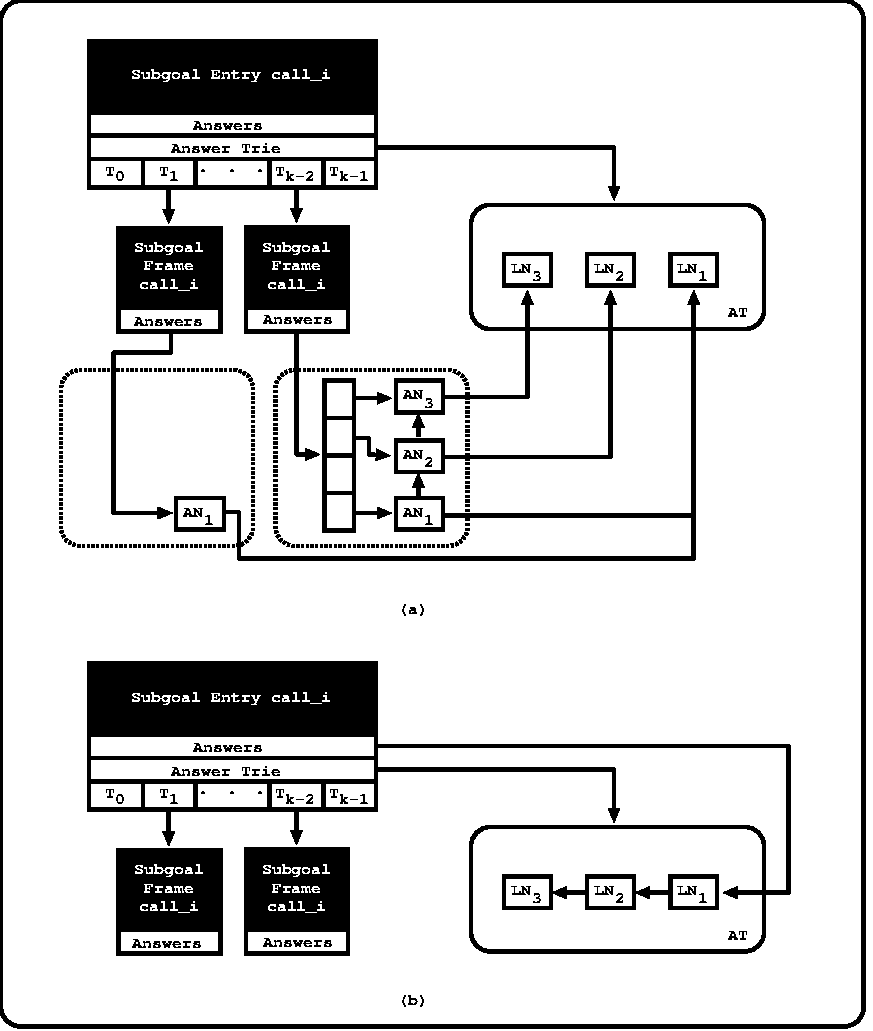
\includegraphics[width=10.5cm]{figures/pcc.pdf}
\caption{The \emph{FS} design with the PAC procedure - (a) private
  chaining and (b) public chaining}
\label{fig_tabtries_pcc}
\end{figure}

Figure~\ref{fig_tabtries_pcc}(a) shows then a situation where two
threads, $T_1$ and $T_{k-1}$, are sharing the same subgoal entry call
$P_{i.j}$ when the subgoal is still under evaluation, i.e., the
subgoal is not yet complete. The current state of the evaluation shows
an answer trie with $3$ answers found for the subgoal call
$P_{i.j}$. For the sake of simplicity, we are omitting the internal
answer trie nodes and we are only showing the leaf nodes nodes $LN_1$,
$LN_2$ and $LN_3$, in the figure. With the PAC procedure, the leaf
nodes are not chained in the \emph{AT} data structure. Now, the
chaining process is done privately, and for that, we use the subgoal
frame structure of each thread. On the subgoal frame structure we
added a new field, called \emph{consumer}, to store the answers found
within the execution of the thread. In order to minimize the impact of
the \emph{PAC} optimization, each node within the new consumer answer
structure has two fields: (i) an entry pointer, which points to the
corresponding leaf node in the answer trie data structure; (ii) a next
pointer to chain the answers within the consumer structure. To
maintain a good performance, when the number of nodes exceeds a
certain threshold, we use a hash trie mechanism design similar to the
one presented in the work~\cite{Areias-ijpp15}. However, since this
mechanism is private to each thread, it does not require any of the
tools that were necessary to support concurrency. In particular, on
each hash trie level, we have removed the tools necessary to support
concurrency, such as useless pointers and compare-and-swap
operations. We have chosen this hashing mechanism, because it showed a
good balance between lookup and insert
operations~\cite{Areias-ijpp15}, but the major reason was mostly
because of the integration in the TabMalloc memory
allocator~\cite{Areias-12b}.

Going back to Figure~\ref{fig_tabtries_pcc}(a), the consumer answer
structures represent then two different situations where threads can
be evaluating a subgoal call. Thread $T_1$ has only found one answer
and it is using a direct consumer answer chaining to access the node
$LN_1$. Thread $T_{k-1}$ was already found three answers for the
subgoal call and it is already using the hash trie mechanism within
its consumer answer structure. The consumer nodes are chained between
themselves, thus that consumer nodes belonging to thread $T_{k-1}$ can
consume the answers as in the original mechanism.

Figure~\ref{fig_tabtries_pcc}(b) shows the state of the subgoal call
after completion (recall that after completion of a subgoal call, the
threads use loader nodes to consume the answers). When a thread $T$
completes a subgoal call, it frees its private consumer structures,
but before doing that, it checks whether another thread as already
marked the subgoal as completed. If no other thread has done that,
then thread $T$ not only follows its private chaining mechanism as it
would for freeing its private nodes, but also, follows the pointers to
the answer trie leaf nodes in order to reproduce the chain inside the
answer trie. Since this procedure is done inside a critical region, no
more than one thread can be doing this chaining process. Thus, in
Figure~\ref{fig_tabtries_pcc}(b), we are showing a situation where the
subgoal call is completed and both threads $T_1$ and $T_{k-1}$ have
already removed their consumer answer structures and chained the leaf
nodes inside the answer trie.

%%%%%%%%%%%%%%%%%%%%%%%%%%%%%%%%%%%%%%%%%%%%%%%%%%%%%%%%%%%%%%%%%%%%%%
\subsection{Implementations details}

At the implementation level, the major difference between local and
batched scheduling is in the tabling operation \emph{tabled new
  answer}, where we decide what to do when an answer is found during
the evaluation. This operation checks whether a newly found answer is
already in the corresponding answer trie structure and, if not,
inserts it. For the NS and SS designs the support for batched
scheduling is immediate, since the answer trie data structure is not
shared among threads. The usage of batched scheduling with the FS
design requires further support since with batched scheduling, answers
are immediately propagated and we have to ensure that the propagation
of an answer occurs on all subgoal calls one and only once. To do so,
we take advantage of the private chaining procedure, presented in the
previous subsection, as a way to keep, for every subgoal call of every
thread, track of all the answers that were already propagated. This
requires minor changes to the \emph{tabled new answer} tabling
operation. Algorithm~\ref{alg_table_new_answer_batched} shows how we
have extended the tabled new answer operation to support the FS design
with batched scheduling.

\begin{algorithm} [ht]
\caption{tabled\_new\_answer(answer ANS, subgoal frame SF)}
\algsetup{indent=0.65cm}
\begin{algorithmic}[1]
  \STATE $leaf \gets check\_insert\_answer\_trie(ANS, SF)$
  \IF {$NS\_design\ or\ SS\_design$}
    \STATE $. . .$                         \COMMENT{without changes}
  \ELSE                                                  [FS design]
    \STATE $chain \gets check\_insert\_consumer\_chain(leaf, SF)$
    \IF {$is\_answer\_marked\_as\_found(chain) = True$}
      \RETURN $failure$
     \ELSE                                        [the answer is new]
       \STATE $mark\_answer\_as\_found(chain)$
       \IF {$local\_scheduling\_mode(SF)$}
         \RETURN $failure$
       \ELSE                                    [batched scheduling mode]
         \RETURN $proceed$
       \ENDIF
     \ENDIF
   \ENDIF
\end{algorithmic}
\label{alg_table_new_answer_batched}
\end{algorithm}

The algorithm receives two arguments: the new answer found during the
evaluation (\emph{ANS}) and the subgoal frame which corresponds to the
call at hand (\emph{SF}). The \emph{NS\_design}, \emph{SS\_design} and
\emph{FS\_design} macros define which table design is enabled.

The algorithm begins by checking/inserting the given \emph{ANS} into
the answer trie structure, which will return the leaf node for the
path representing \emph{ANS} (line 1). In line 2, it then tests
whether one of the NS or SS designs are active, and in such a case,
the algorithm is remains unchanged.

Otherwise, for the FS design (lines 4 to 13), it checks/inserts
the given \emph{leaf} node into the private consumer chain for the
current thread, which will return the corresponding chain node. In
line 6, it then tests whether the chain node already existed in the
consumer chain, i.e., if it was inserted or not by the current
check/insert operation in order to return failure (line 7), or it
proceed with marking the answer \emph{ANS} has found (line 9). At the
end (lines 10 to 13), it returns failure if local scheduling is active
(line 11), otherwise, the batched scheduling is active, thus it
propagates the answer \emph{ANS} (line 13).

%%%%%%%%%%%%%%%%%%%%%%%%%%%%%%%%%%%%%%%%%%%%%%%%%%%%%%%%%%%%%%%%%%%%%%
\section{Performance Analysis}

We now present experimental results about the usage of the batched
scheduling on the \emph{NS}, \emph{SS} and \emph{FS} designs. The
environment for our experiments was a machine with 32-Core AMD Opteron
(TM) Processor 6274 (2 sockets with 16 cores each) with 32G of main
memory, each processor with caches $L1$, $L2$ and $L3$ respectively
with the sizes of 64K, 2048K and 6144K, running the Linux kernel is
the 3.16.7-200.fc20.x86\_64, with Yap 6.3 compiled with gcc 4.8.

We used five sets of benchmarks. The \emph{Large Joins} and
\emph{WordNet} sets were obtained from the OpenRuleBench
project~\cite{Liang-09}; the \emph{Model Checking} set includes three
different specifications and transition relation graphs usually used
in model checking applications; the \emph{Path Left} and \emph{Path
  Right} sets implement two recursive definitions of the well-known
$path/2$ predicate, that computes the transitive closure in a graph,
using several different configurations of $edge/2$ facts. We
experimented graphs with the \emph{BTree} configuration with depth 17,
the \emph{Pyramid} and \emph{Cycle} configurations with depth 2000 and
the \emph{Grid} configuration with depth 35. 

In order to have a deeper insight on the behavior of each benchmark,
and therefore clarify some of the results that are presented next, we
first characterize the benchmarks. The columns in
Table~\ref{tab_benchs} have the following meaning: (i) {\bf calls:} is
the number of different calls to tabled subgoals. It corresponds to
the number of paths in the subgoal tries. (ii) {\bf trie nodes:} is
the total number of trie nodes allocated in the corresponding
subgoal/answer trie structures. (iii) {\bf trie depth:} is the
minimum/average/maximum number of trie node levels required to
represent a path in the corresponding subgoal/answer trie
structures. Trie structures with smaller average values are more
amenable to higher lock contention. (iv) {\bf unique:} is the number
of different tabled answers found. It corresponds to the number of
paths in the answer tries. (v) {\bf repeated:} is the number of
redundant tabled answers found. (vi) {\bf NS:} is the average
execution time, in seconds, of ten runs for 1 thread with the NS
design without the TabMalloc memory allocator. In what follows, we
will use these times as the base times when computing the overhead
ratios for the other designs.

By observing Table~\ref{tab_benchs}, the \emph{Mondial} benchmark,
from the \emph{Large Joins} set, and the three \emph{Model
  Checking} benchmarks seem to be the benchmarks least amenable to
lock contention since they are the ones that find less unique answers
and that have the deepest trie structures. In this regard, the
\emph{Path Left} and \emph{Path Right} sets correspond to the
opposite case. They find a huge number of answers and have very
shallow trie structures. On the other hand, the \emph{WordNet} and
\emph{Path Right} sets have the benchmarks with the largest number
of different subgoal calls, which can reduce the probability of lock
contention because answers can be found for different subgoal calls
and therefore be inserted with minimum overlap. On the opposite side
are the \emph{Join2} benchmark, from the \emph{Large Joins} set,
and the \emph{Path Left} benchmarks, which have only a single tabled
subgoal call.

\begin{table}[ht]
\centering
\caption{Characteristics of the benchmark programs}
\scalebox{0.82} { 
\begin{tabular}{lrrccrrrcc}
\hline\hline
\multirow{2}{*}{\bf Bench}
& \multicolumn{3}{c}{\bf Tabled Subgoals}
&
& \multicolumn{4}{c}{\bf Tabled Answers}
& \multicolumn{1}{c}{\bf Time (sec)} \\ \cline{2-4}\cline{6-9}
& \multicolumn{1}{c}{\bf calls}
& \multicolumn{1}{c}{\bf trie nodes}
& \multicolumn{1}{c}{\bf trie depth}
&
& \multicolumn{1}{c}{\bf unique}
& \multicolumn{1}{c}{\bf repeated}
& \multicolumn{1}{c}{\bf trie nodes}
& \multicolumn{1}{c}{\bf trie depth}
& \multicolumn{1}{c}{\bf NS} \\
\hline
\multicolumn{10}{l}{\bf Large Joins} \\
\bf{Join2}    &       1 &       6 & 5/5/5 && 2,476,099 &         0 &
2,613,660 &    5/5/5 &  2.85 \\
\bf{Mondial}  &      35 &      42 & 3/4/4 &&     2,664 & 2,452,890 &
   14,334 &    6/7/7 &  0.84 \\
\hline
\multicolumn{10}{l}{\bf WordNet} \\
\bf{Clusters} & 117,659 & 235,319 & 2/2/2 &&   166,877 &   161,853 &
284,536 &    1/1/1 &   0.83 \\
\bf{Holo}     & 117,657 & 235,315 & 2/2/2 &&    74,838 &        54 &
192,495 &    1/1/1 &   0.75 \\
\bf{Hyper}    & 117,657 & 235,315 & 2/2/2 &&   698,472 &     8,658 &
816,129 &    1/1/1 &   1.42 \\
\bf{Hypo}     & 117,657 & 117,659 & 2/2/2 &&   698,472 &    20,341 &
816,129 &    1/1/1 &   1.53 \\
\bf{Mero}     & 117,657 & 117,659 & 2/2/2 &&    74,838 &        13 &
192,495 &    1/1/1 &   0.74 \\
\bf{Tropo}    & 117,657 & 235,315 & 2/2/2 &&       472 &         0 &
118,129 &    1/1/1 &   0.66 \\
\hline
\multicolumn{10}{l}{\bf Model Checking} \\
\bf{IProto}   &       1 &       6 & 5/5/5 &&   134,361 &   385,423 &
1,554,896 &  4/51/67 & 2.70 \\
\bf{Leader}   &       1 &       5 & 4/4/4 &&     1,728 &   574,786 &
   41,788 & 15/80/97 & 3.51  \\
\bf{Sieve}    &       1 &       7 & 6/6/6 &&       380 & 1,386,181 &
    8,624 & 21/53/58 & 18.50 \\
\hline
\multicolumn{10}{l}{\bf Path Left} \\
\bf{BTree}    &       1 &       3 & 2/2/2 && 1,966,082 &         0 &
2,031,618 &    2/2/2 &   1.53 \\
\bf{Cycle}    &       1 &       3 & 2/2/2 && 4,000,000 &     2,000 &
4,002,001 &    2/2/2 &   3.52 \\
\bf{Grid}     &       1 &       3 & 2/2/2 && 1,500,625 & 4,335,135 &
1,501,851 &    2/2/2 &  1.93 \\
\bf{Pyramid}  &       1 &       3 & 2/2/2 && 3,374,250 & 1,124,250 &
3,377,250 &    2/2/2 &   3.08 \\
\hline
\multicolumn{10}{l}{\bf Path Right} \\
\bf{BTree}    & 131,071 & 262,143 & 2/2/2 && 3,801,094 &         0 &
3,997,700 &    1/2/2 &  2.33 \\
\bf{Cycle}    &   2,001 &   4,003 & 2/2/2 && 8,000,000 &     4,000 &
8,004,001 &    1/2/2 &  3.55 \\
\bf{Grid}     &   1,226 &   2,453 & 2/2/2 && 3,001,250 & 8,670,270 &
3,003,701 &    1/2/2 &  2.32 \\
\bf{Pyramid}  &   3,000 &   6,001 & 2/2/2 && 6,745,501 & 2,247,001 &
6,751,500 &    1/2/2 &  3.17 \\
\hline\hline
\end{tabular}}
\label{tab_benchs}
\end{table}

Note that for the moment our goal is to evaluate the robustness of our
implementation when exposed to \emph{worst case} scenarios. By
focusing on \emph{worst case} scenarios, we show the lowest bounds in
terms of performance that each design might achieve when applied/used
with other real world applications/programs. Moreover, by testing the
framework with worst case scenarios, we avoid the peculiarities of the
program at hand and we try to focus on measuring the real value of our
designs. Thus, we will follow a common approach to create worst case
scenarios and we will run all threads starting with the same query
goal. By doing this, it is expected that all threads will access the
table space, to check/insert for subgoals and answers, at similar
times, thus causing a huge stress on the same critical regions. To put
the results in perspective, we experimented with $1$, $8$, $16$, $24$
and $32$ threads (the maximum number of cores available in our
machine) with local and batched scheduling on the five sets of
benchmarks presented in the early subsection.

Table~\ref{tab_batched_overhead} shows the overhead ratios, when
compared with the NS design with 1 thread (running with local
scheduling), for the NS, SS and FS designs (all running TabMalloc),
when running 1, 8, 16, 24 and 32 threads with local and batched
scheduling on the five sets of benchmarks. For each design, the table
has then two columns, a column with {\bf Local} that shows results for
the local scheduling and a column with {\bf Batched} with results for
batched scheduling. The overhead results presented in both {\bf Local}
and {\bf Batched} columns use as base time the execution times
presented in the {\bf NS} column of the Table~\ref{tab_benchs}.

\begin{table}[!ht]
\centering
\caption{Overhead ratios, when compared with the NS design with $1$
  thread (running with local scheduling without TabMalloc) for the NS,
  SS, FS designs (with TabMalloc), when running 1, 8, 16, 24 and 32
  threads with local and batched scheduling on the five sets of
  benchmarks (best ratios by row and by design for the Minimum,
  Average and Maximum are in bold)}
%\scalebox{1.00} {
\begin{tabular}{ll|cc|cc|cc}
\hline\hline
\multicolumn{2}{c|}{\multirow{2}{*}{\bf Threads}} &
\multicolumn{2}{c|}{\multirow{1}{*}{\bf NS}} &
\multicolumn{2}{c}{\multirow{1}{*}{\bf SS}} & 
\multicolumn{2}{|c}{\multirow{1}{*}{\bf FS}}\\ \cline{3-8}
& 
& \multicolumn{1}{c}{\bf Local}
& \multicolumn{1}{c}{\bf Batched}
& \multicolumn{1}{|c}{\bf Local}
& \multicolumn{1}{c}{\bf Batched}
& \multicolumn{1}{|c}{\bf Local}
& \multicolumn{1}{c}{\bf Batched}\\
\hline
\multirow{4}{*}{\bf 1}
& {\bf Min }& {\bf 0.53}& 0.55& {\bf 0.54}& 0.55& 1.01& {\bf 0.95}\\
& {\bf Avg }& {\bf 0.78}& 0.82& {\bf 0.84}& 0.90& {\bf 1.30}& 1.46\\
& {\bf Max }& 1.06& {\bf 1.05}& {\bf 1.04}& {\bf 1.04}& {\bf 1.76}& 2.33\\
& {\bf StD }& 0.15& 0.14& 0.17& 0.16& 0.22& 0.44\\
\hline
\multirow{4}{*}{\bf 8}
& {\bf Min }& 0.66& {\bf 0.63}& 0.66& {\bf 0.63}& 1.16&{\bf  0.99}\\
& {\bf Avg }& {\bf 0.85}& 0.88& {\bf 0.92}& 0.93& {\bf 1.88}& 1.95\\
& {\bf Max }& {\bf 1.12}& 1.14& 1.20& {\bf 1.15}& {\bf 2.82}& 3.49\\
& {\bf StD }& 0.13& 0.14& 0.15& 0.14& 0.60& 0.79\\
\hline
\multirow{4}{*}{\bf 16}
& {\bf Min }& 0.85& {\bf 0.75}& 0.82& {\bf 0.77}& 1.17& {\bf 1.06}\\
& {\bf Avg }& {\bf 0.98}& 1.00& {\bf 1.04}& 1.05& {\bf 1.97}& 2.08\\
& {\bf Max }& {\bf 1.16}& 1.31& 1.31& {\bf 1.28}& {\bf 3.14}& 3.69\\
& {\bf StD }& 0.09& 0.17& 0.12& 0.13& 0.65& 0.83\\
\hline
\multirow{4}{*}{\bf 24}
& {\bf Min }& {\bf 0.91}& 0.93& 1.02& {\bf 0.98}& 1.16& {\bf 1.09}\\
& {\bf Avg }& {\bf 1.15}& 1.16& 1.22& {\bf 1.19}& {\bf 2.06}& 2.19\\
& {\bf Max }& 1.72& {\bf 1.60}& 1.81& {\bf 1.61}& {\bf 3.49}& 4.08\\
& {\bf StD }& 0.20& 0.21& 0.18& 0.16& 0.70& 0.91\\
\hline
\multirow{4}{*}{\bf 32}
& {\bf Min }& 1.05& {\bf 1.04}& {\bf 1.07}& 1.12& 1.33& {\bf 1.26}\\
& {\bf Avg }& 1.51& {\bf 1.49}& 1.54& {\bf 1.51}& {\bf 2.24}& 2.41\\
& {\bf Max }& {\bf 2.52}& 2.63& {\bf 2.52}& 2.62& {\bf 3.71}& 4.51\\
& {\bf StD }& 0.45& 0.45& 0.42& 0.43& 0.74& 1.02\\
\hline\hline
\end{tabular}%}
\label{tab_batched_overhead}
\end{table}

By observing Table~\ref{tab_batched_overhead}, we can see that, for
one thread, on average, local scheduling is sightly better than
batched on the three designs. For the NS design we have $0.78$ and
$0.82$, for the SS design we have $0.84$ and $0.90$ and for the FS
design we have $1.30$ and $1.46$ average overhead ratios, for the
local and batched scheduling strategies, respectively. As we scale the
number of threads, one can observe that, for the NS and SS designs
both scheduling strategies have similar minimum, average and maximum
overhead ratios. For the FS design, the best minimum overhead ratio is
always for batched scheduling. For the average and maximum overhead
ratio, local scheduling is always better than batched scheduling. In
summary, we can say that both the local and batched scheduling
strategies have similar overhead results on worst case scenarios for
the NS, SS and FS designs.


%%%%%%%%%%%%%%%%%%%%%%%%%%%%%%%%%%%%%%%%%%%%%%%%%%%%%%%%%%%%%%%%%%%%%%
\section{Conclusions and Further Work}

%%%%%%%%%%%%%%%%%%%%%%%%%%%%%%%%%%%%%%%%%%%%%%%%%%%%%%%%%%%%%%%%%%%%%%

%\section*{Acknowledgments}

%%%%%%%%%%%%%%%%%%%%%%%%%%%%%%%%%%%%%%%%%%%%%%%%%%%%%%%%%%%%%%%%%%%%%%

\bibliographystyle{splncs}
\bibliography{references}

%%%%%%%%%%%%%%%%%%%%%%%%%%%%%%%%%%%%%%%%%%%%%%%%%%%%%%%%%%%%%%%%%%%%%%

\end{document}
